\chapter{Design}
\label{cha:design}
Implementing any kind of simulation or emulation can be done in various structures and designs which can be tailored for specific requirements.
Given an existing system different questions regarding the complexity of modules and the designed hierarchy are brought up.
Such a given system can be an existing application or other given functionalities, which must be embedded within the simulation without changing the original system.
The following sections will discuss two fundamental design strategies and their impact on development and achievable results.
Furthermore the according functionalities and strategies within OMNeT++ are explained.
An according example simulation and the resulting performances are shown and discussed in chapter \ref{cha:measurements}.

\section{Modular design}
\label{sec:design_modular}
A modular design implies a bigger number of different components communicating with each other.
Different functional units from the original system are represented by the composition of multiple components and their interactions.
This approach can lead to a more dynamic simulation and increase the reusability of different components and modules.
Developing a complex systems can also be eased by using a modular design and therefore an increased separation in smaller functional units.

A modular design can also provide more insight in a given system and the executed procedures.
This increased insight can be used for educational and exemplary usages showing detailed informations about the internal procedures of a functional unit.
During development of the simulation or the simulated system a modular design can also provide more insight and therefore improved analyzing and debugging possibilities.
The increased number of simulated components and the separation of functionality compared to a monolithic design results in increased communication between components.

Designing a modular system in OMNeT++ is done by implementing a bigger number of modules connected with channels and grouped in compound modules.
A simulated network consisting of multiple modules and therefore implementing a modular design results in increased communication, i.e. message allocation, transmission and deallocation.
These additional procedures can strongly influence the achievable performance and must be analyzed carefully.

An example of a modular design using OMNeT++ components is shown in figure \ref{fig:OMNeTModularDesign}.
This example contains multiple compound modules consisting of enclosed simple and compound modules.
The multiple connections in between the modules show the required communication.

\begin{figure}
    \centering
    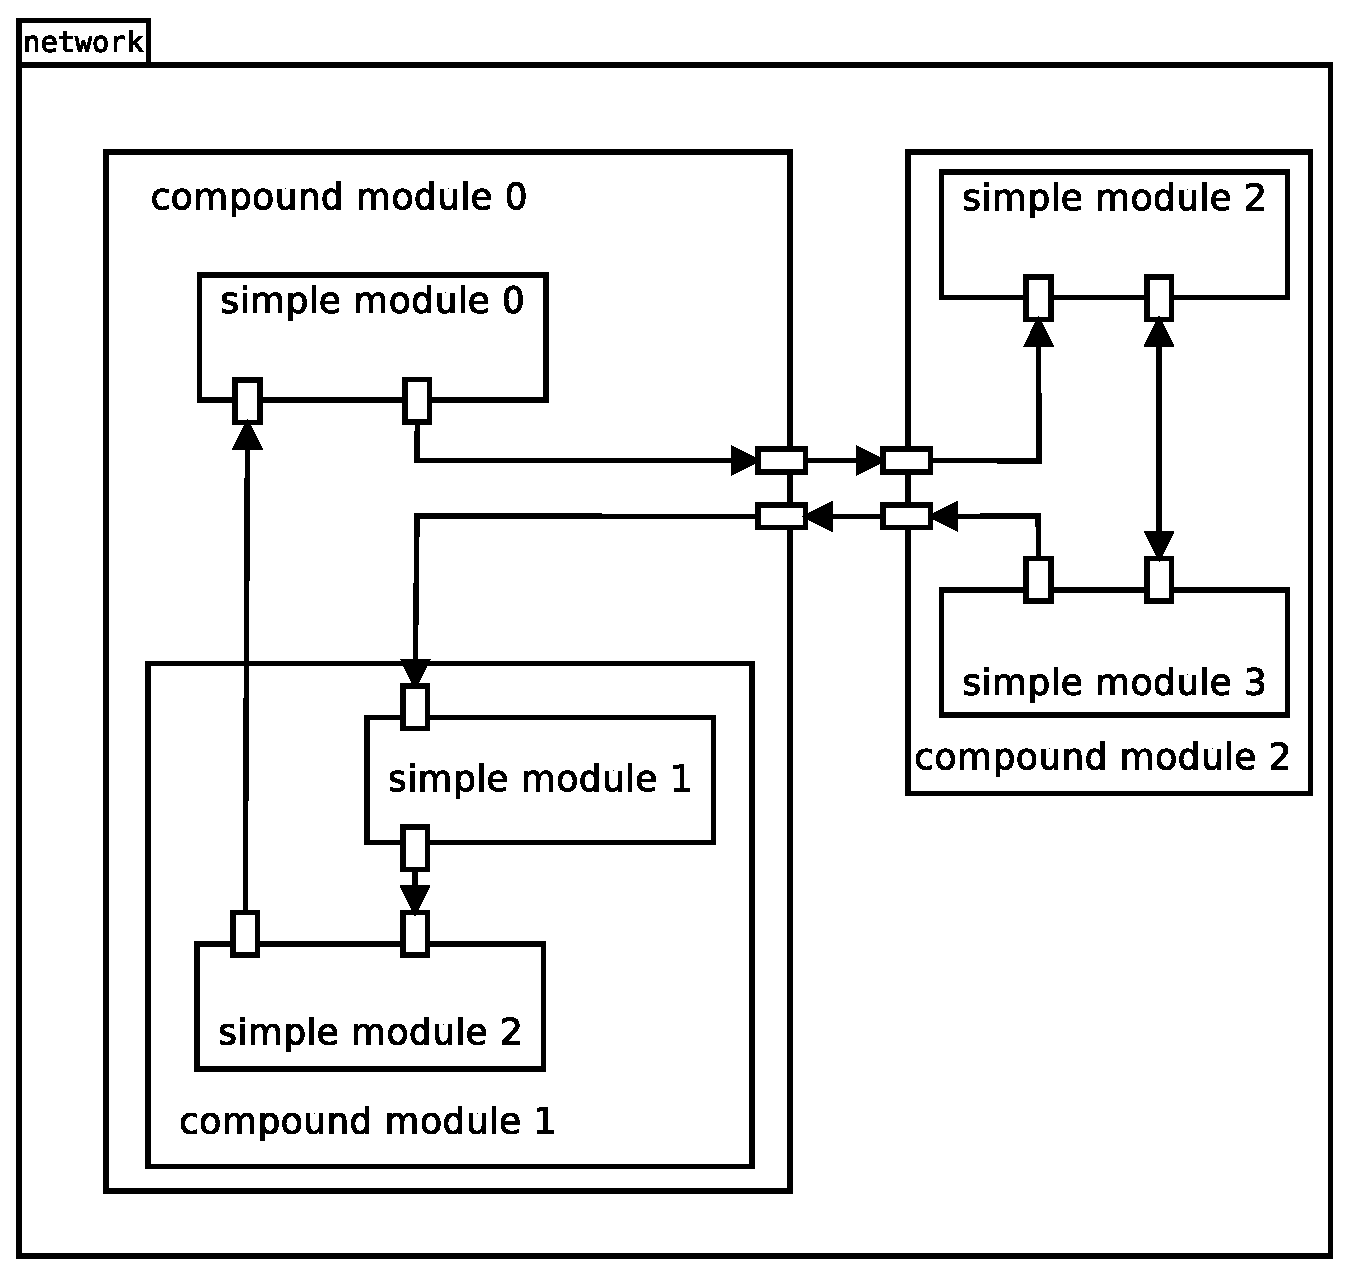
\includegraphics[width=0.8\columnwidth]{OMNeTModularDesign.eps}
    \caption{Modular design with OMNeT++}
    \label{fig:OMNeTModularDesign}
\end{figure}

Approaching the fields of emulation and \emph{HiL} using real-time simulation these design decisions are important for the achieved timings.

As described in section \ref{sec:parallel_omnet} OMNeT++ provides functionalities for running a parallelized simulation and therefore increase the performance by parallelism.
This type of executing is depending strongly on the simulated system and the applied design.
Due to the necessary communication between parallel simulated modules a modular design provides more possibilities for parallelism than a monolithic design.

Developing a simulation for a given system with an existing implementation results in restraints for the applicable design.
The simulation of a system which shows a modular structure can also be designed modular using the separations of the given system.
For a modular designed simulation the connection of simulated system and according simulation modules must be possible.
This connection can be achieved when the existing system is already using interfaces or function pointer for the connections of different components.
These communication parts can be used for redirecting calls to wrapper modules embedding the simulated system in the simulation environment.
These modules handle all received messages, forward them to the enclosed component and create necessary outgoing messages.
The enclosed component can be instanced within the wrapper module and therefore embedded in the simulation.

\section{Monolithic design}
\label{sec:design_monolithic}
The opposite approach to the modular design discussed in the previous section is the monolithic design.
A monolithic design implies a lower number of components, but an increased functionality within a single one.
This decreased number of components lower the necessary communication and a potential overhead.
The reduced modularity does not allow deep insight in the system but can result in improved performance.
Is a simulated system used as a single functional unit and maybe even instanced multiple times within the simulation a monolithic design is favorable, especially when no detailed information about internal procedures is demanded.

Within OMNeT++ a monolithic design can be achieved by condensing a compound module to a simple module with more complex functions.
The execution of the single modules include more normal C++ code using simple method calls and operations.
This can be done via enclosing multiple components of the given system within a single simple module.
Such components can be connected directly to each other, such as the normal execution regardless the simulation environment.
The surrounding module must, similar to the implementation of modular wrapper modules, handle and forward incoming messages or create outgoing messages for the communication with the remaining simulation.

The previous example network showing a modular design in figure \ref{fig:OMNeTModularDesign} can be condensed to a more monolithic design.
In the example, shown in figure \ref{fig:OMNeTMonolithicDesign}, the compound modules 0 and 2 with all their submodules were replaced by two simple modules.
The channels and the sent messages between the modules stay the same, but the calculation within the modules include the complete behavior of the previously included components.

\begin{figure}
    \centering
    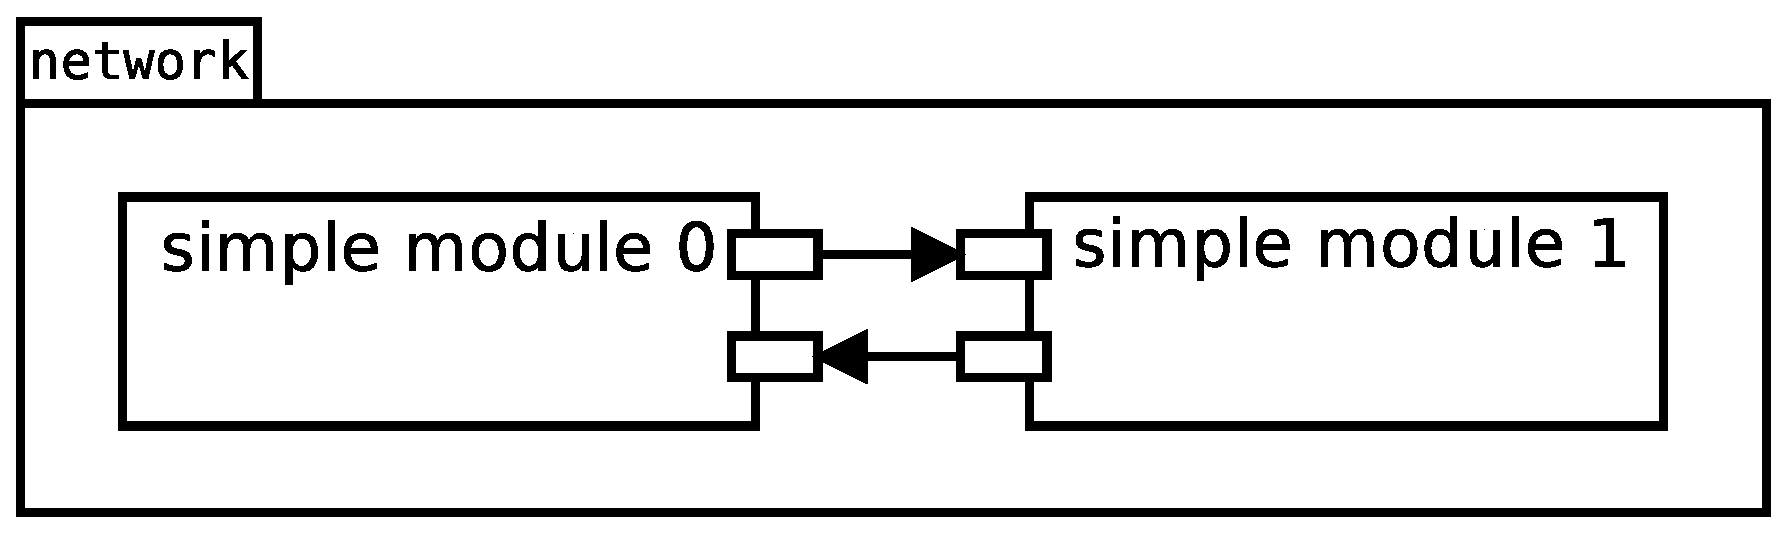
\includegraphics[width=0.8\columnwidth]{OMNeTMonolithicDesign.eps}
    \caption{Monolithic design with OMNeT++}
    \label{fig:OMNeTMonolithicDesign}
\end{figure}

As mentioned in this and the previous chapter a parallelized simulation can provide improved behavior and benefit from specific designs.
The properties of a parallel simulation and the provided functionalities of OMNeT++ are analyzed in the next chapter.